%--------------------
% Packages
% -------------------
\documentclass[11pt,english]{article}
\usepackage{amsfonts}
\usepackage[left=2.5cm,top=2cm,right=2.5cm,bottom=3cm,bindingoffset=0cm]{geometry}
\usepackage{amsmath, amsthm, amssymb}
\usepackage{tikz}
\usetikzlibrary{calc}
\usetikzlibrary{decorations.pathreplacing,calligraphy}
\usepackage{fancyhdr}
%\usepackage{currfile}
\usepackage{nicefrac}
\usepackage{cite}
\usepackage{graphicx}
\usepackage{caption}
\usepackage{longtable}
\usepackage{rotating}
\usepackage{lscape}
\usepackage{booktabs}
\usepackage{float}
\usepackage{placeins}
\usepackage{setspace}
\usepackage[font=itshape]{quoting}
\onehalfspacing
\usepackage{mathrsfs}
\usepackage{tcolorbox}
\usepackage{xcolor}
\usepackage{subcaption}
\usepackage{float}
\usepackage[multiple]{footmisc}
\usepackage[T1]{fontenc}
\usepackage[sc]{mathpazo}
\usepackage{listings}
\usepackage{longtable}
\definecolor{cmured}{RGB}{175,30,45}
\definecolor{macroblue}{RGB}{56,108,176}
\usepackage[format=plain,
            labelfont=bf,
            textfont=]{caption}
\usepackage[colorlinks=true,citecolor=macroblue,linkcolor=macroblue,urlcolor=macroblue]{hyperref}
\usepackage{varioref}
\usepackage{chngcntr}
\usepackage{datetime}

\definecolor{darkgreen}{RGB}{30,175,88}
\definecolor{darkblue}{RGB}{30,118,175}
\definecolor{maroon}{rgb}{0.66,0,0}
\definecolor{darkgreen}{rgb}{0,0.69,0}

%Counters
\newtheorem{theorem}{Theorem}[section] 
\newtheorem{proposition}{Proposition}
\newtheorem{lemma}{Lemma}
\newtheorem{corollary}{Corollary}
\newtheorem{assumption}{Assumption}
\newtheorem{axiom}{Axiom}
\newtheorem{case}{Case}
\newtheorem{claim}{Claim}
\newtheorem{condition}{Condition}
\newtheorem{definition}{Definition}
\newtheorem{example}{Example}
\newtheorem{notation}{Notation}
\newtheorem{remark}{Remark}


\hypersetup{ 	
pdfsubject = {},
pdftitle = {TidyTuesday Week 1},
pdfauthor = {Pranay Gundam},
linkcolor= macroblue
}


\title{\textbf{TidyTuesday Week 1}}
\author{Pranay Gundam}


%-----------------------
% Begin document
%-----------------------
\begin{document}

\maketitle

\tableofcontents

\section{Weekly Summary}


\section{Date: 2024-12-30}
\noindent \textbf{Series ID: MORTMRGN1NC} 

\noindent This series is titled Margin for 1-Year Adjustable Rate Mortgage in the North Central Freddie Mac Region (DISCONTINUED) and has a frequency of Weekly, Ending Thursday. The units are Percent and the seasonal adjustment is Not Seasonally Adjusted.The observation start date is 1988-02-19 and the observation end date is 2015-12-31.The popularity of this series is 1. \\ 

\noindent \textbf{Series ID: MORTPTS5SW} 

\noindent This series is titled Origination Fees and Discount Points for 5/1-Year Adjustable Rate Mortgage in the Southwest Freddie Mac Region (DISCONTINUED) and has a frequency of Weekly, Ending Thursday. The units are Percent and the seasonal adjustment is Not Seasonally Adjusted.The observation start date is 2005-01-06 and the observation end date is 2015-12-31.The popularity of this series is 1. \\ 

\subsection{Regression Tables and Plots}
\begin{center}
\begin{tabular}{lclc}
\toprule
\textbf{Dep. Variable:}           & value\_fred\_MORTPTS5SW & \textbf{  R-squared:         } &     0.009   \\
\textbf{Model:}                   &           OLS           & \textbf{  Adj. R-squared:    } &     0.007   \\
\textbf{Method:}                  &      Least Squares      & \textbf{  F-statistic:       } &     5.064   \\
\textbf{Date:}                    &     Mon, 30 Dec 2024    & \textbf{  Prob (F-statistic):} &   0.0248    \\
\textbf{Time:}                    &         15:16:10        & \textbf{  Log-Likelihood:    } &    330.55   \\
\textbf{No. Observations:}        &             573         & \textbf{  AIC:               } &    -657.1   \\
\textbf{Df Residuals:}            &             571         & \textbf{  BIC:               } &    -648.4   \\
\textbf{Df Model:}                &               1         & \textbf{                     } &             \\
\textbf{Covariance Type:}         &        nonrobust        & \textbf{                     } &             \\
\bottomrule
\end{tabular}
\begin{tabular}{lcccccc}
                                  & \textbf{coef} & \textbf{std err} & \textbf{t} & \textbf{P$> |$t$|$} & \textbf{[0.025} & \textbf{0.975]}  \\
\midrule
\textbf{const}                    &       1.7796  &        0.528     &     3.370  &         0.001        &        0.742    &        2.817     \\
\textbf{value\_fred\_MORTMRGN1NC} &      -0.4319  &        0.192     &    -2.250  &         0.025        &       -0.809    &       -0.055     \\
\bottomrule
\end{tabular}
\begin{tabular}{lclc}
\textbf{Omnibus:}       &  3.696 & \textbf{  Durbin-Watson:     } &    0.593  \\
\textbf{Prob(Omnibus):} &  0.158 & \textbf{  Jarque-Bera (JB):  } &    3.771  \\
\textbf{Skew:}          &  0.183 & \textbf{  Prob(JB):          } &    0.152  \\
\textbf{Kurtosis:}      &  2.844 & \textbf{  Cond. No.          } &     289.  \\
\bottomrule
\end{tabular}
%\caption{OLS Regression Results}
\end{center}

Notes: \newline
 [1] Standard Errors assume that the covariance matrix of the errors is correctly specified.

\begin{figure}
\centering
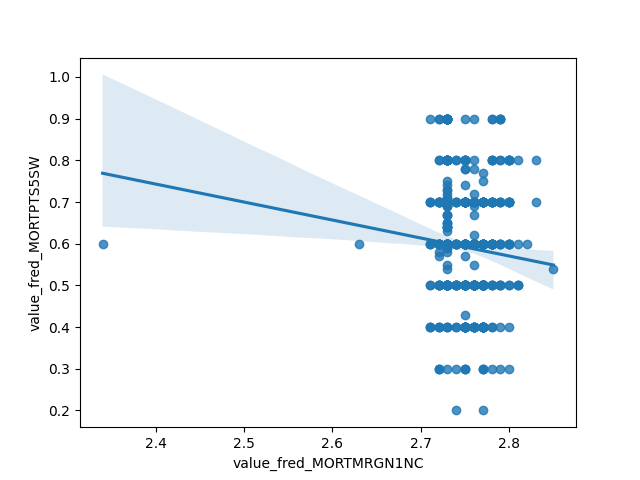
\includegraphics[scale = 0.9]{plots/plot_2024-12-30.png}
\caption{Regression Plot for 2024-12-30}
\end{figure}
\newpage

\section{Date: 2024-12-31}
\noindent \textbf{Series ID: RTFPNABFA632NRUG} 

\noindent This series is titled Total Factor Productivity at Constant National Prices for Burkina Faso and has a frequency of Annual. The units are Index 2017=1 and the seasonal adjustment is Not Seasonally Adjusted.The observation start date is 1963-01-01 and the observation end date is 2019-01-01.The popularity of this series is 1. \\ 

\noindent \textbf{Series ID: PATENT4NSGDESIGN} 

\noindent This series is titled U.S. Granted Patents: Design Patents Originating in Singapore and has a frequency of Annual. The units are Number and the seasonal adjustment is Not Seasonally Adjusted.The observation start date is 1992-01-01 and the observation end date is 2020-01-01.The popularity of this series is 1. \\ 

\subsection{Regression Tables and Plots}
\begin{center}
\begin{tabular}{lclc}
\toprule
\textbf{Dep. Variable:}                & value\_fred\_PATENT4NSGDESIGN & \textbf{  R-squared:         } &     0.565   \\
\textbf{Model:}                        &              OLS              & \textbf{  Adj. R-squared:    } &     0.548   \\
\textbf{Method:}                       &         Least Squares         & \textbf{  F-statistic:       } &     33.74   \\
\textbf{Date:}                         &        Tue, 31 Dec 2024       & \textbf{  Prob (F-statistic):} &  4.04e-06   \\
\textbf{Time:}                         &            22:43:33           & \textbf{  Log-Likelihood:    } &   -117.61   \\
\textbf{No. Observations:}             &                 28            & \textbf{  AIC:               } &     239.2   \\
\textbf{Df Residuals:}                 &                 26            & \textbf{  BIC:               } &     241.9   \\
\textbf{Df Model:}                     &                  1            & \textbf{                     } &             \\
\textbf{Covariance Type:}              &           nonrobust           & \textbf{                     } &             \\
\bottomrule
\end{tabular}
\begin{tabular}{lcccccc}
                                       & \textbf{coef} & \textbf{std err} & \textbf{t} & \textbf{P$> |$t$|$} & \textbf{[0.025} & \textbf{0.975]}  \\
\midrule
\textbf{const}                         &    -104.7271  &       24.257     &    -4.317  &         0.000        &     -154.589    &      -54.865     \\
\textbf{value\_fred\_RTFPNABFA632NRUG} &     149.7860  &       25.788     &     5.808  &         0.000        &       96.778    &      202.794     \\
\bottomrule
\end{tabular}
\begin{tabular}{lclc}
\textbf{Omnibus:}       &  2.778 & \textbf{  Durbin-Watson:     } &    1.137  \\
\textbf{Prob(Omnibus):} &  0.249 & \textbf{  Jarque-Bera (JB):  } &    1.550  \\
\textbf{Skew:}          &  0.540 & \textbf{  Prob(JB):          } &    0.461  \\
\textbf{Kurtosis:}      &  3.402 & \textbf{  Cond. No.          } &     15.3  \\
\bottomrule
\end{tabular}
%\caption{OLS Regression Results}
\end{center}

Notes: \newline
 [1] Standard Errors assume that the covariance matrix of the errors is correctly specified.

\begin{figure}
\centering
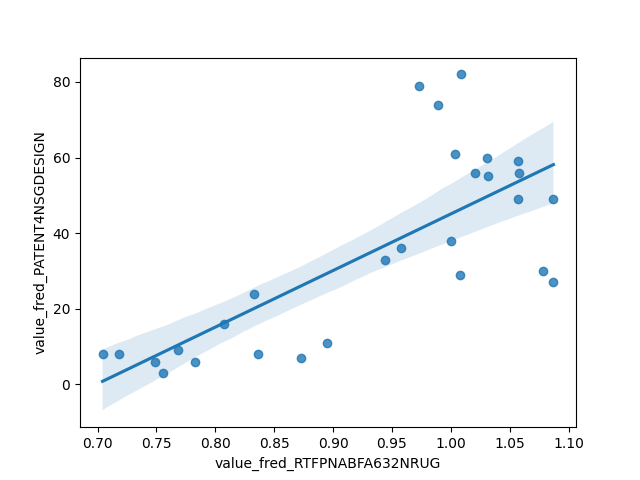
\includegraphics[scale = 0.9]{plots/plot_2024-12-31.png}
\caption{Regression Plot for 2024-12-31}
\end{figure}
\newpage

\include{tex_things/day_2025-01-01}
\section{Date: 2025-01-02}
\noindent \textbf{Series ID: WPDILVA} 

\noindent This series is titled Discussion About Pandemics Index for Latvia and has a frequency of Quarterly. The units are Index and the seasonal adjustment is Not Seasonally Adjusted.The observation start date is 1996-01-01 and the observation end date is 2024-07-01.The popularity of this series is 1. \\ 

\noindent \textbf{Series ID: CCDIOA17140Q156N} 

\noindent This series is titled CredAbility Consumer Distress Index for Cincinnati-Middletown, OH-KY-IN (MSA) (DISCONTINUED) and has a frequency of Quarterly. The units are Percent and the seasonal adjustment is Not Seasonally Adjusted.The observation start date is 2005-01-01 and the observation end date is 2013-01-01.The popularity of this series is 0. \\ 

\subsection{Regression Tables and Plots}
\begin{center}
\begin{tabular}{lclc}
\toprule
\textbf{Dep. Variable:}       & value\_fred\_CCDIOA17140Q156N & \textbf{  R-squared:         } &     0.000   \\
\textbf{Model:}               &              OLS              & \textbf{  Adj. R-squared:    } &     0.000   \\
\textbf{Method:}              &         Least Squares         & \textbf{  F-statistic:       } &       nan   \\
\textbf{Date:}                &        Thu, 02 Jan 2025       & \textbf{  Prob (F-statistic):} &      nan    \\
\textbf{Time:}                &            10:10:29           & \textbf{  Log-Likelihood:    } &   -94.269   \\
\textbf{No. Observations:}    &                 33            & \textbf{  AIC:               } &     190.5   \\
\textbf{Df Residuals:}        &                 32            & \textbf{  BIC:               } &     192.0   \\
\textbf{Df Model:}            &                  0            & \textbf{                     } &             \\
\textbf{Covariance Type:}     &           nonrobust           & \textbf{                     } &             \\
\bottomrule
\end{tabular}
\begin{tabular}{lcccccc}
                              & \textbf{coef} & \textbf{std err} & \textbf{t} & \textbf{P$> |$t$|$} & \textbf{[0.025} & \textbf{0.975]}  \\
\midrule
\textbf{const}                &      71.4297  &        0.744     &    95.956  &         0.000        &       69.913    &       72.946     \\
\textbf{value\_fred\_WPDILVA} &            0  &            0     &       nan  &           nan        &            0    &            0     \\
\bottomrule
\end{tabular}
\begin{tabular}{lclc}
\textbf{Omnibus:}       & 10.222 & \textbf{  Durbin-Watson:     } &    0.253  \\
\textbf{Prob(Omnibus):} &  0.006 & \textbf{  Jarque-Bera (JB):  } &    2.567  \\
\textbf{Skew:}          &  0.159 & \textbf{  Prob(JB):          } &    0.277  \\
\textbf{Kurtosis:}      &  1.671 & \textbf{  Cond. No.          } &      inf  \\
\bottomrule
\end{tabular}
%\caption{OLS Regression Results}
\end{center}

Notes: \newline
 [1] Standard Errors assume that the covariance matrix of the errors is correctly specified. \newline
 [2] The smallest eigenvalue is      0. This might indicate that there are \newline
 strong multicollinearity problems or that the design matrix is singular.

\begin{figure}
\centering
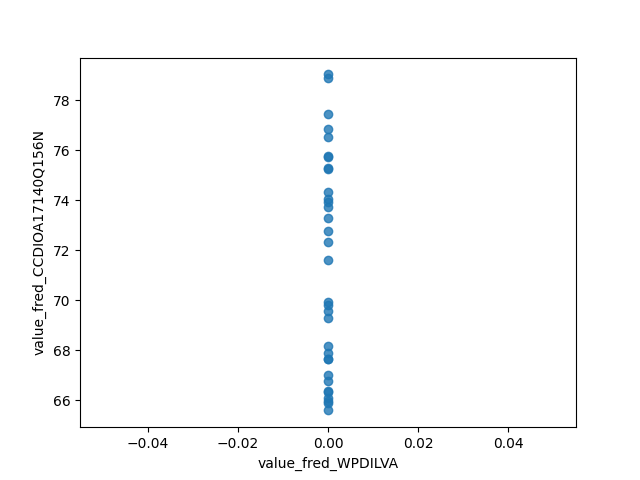
\includegraphics[scale = 0.9]{plots/plot_2025-01-02.png}
\caption{Regression Plot for 2025-01-02}
\end{figure}
\newpage

\include{tex_things/day_2025-01-03}
\include{tex_things/day_2025-01-04}
\include{tex_things/day_2025-01-05}

\end{document}
